\section{Background}

People spend more time than ever using computing devices. Work, entertainment, and services, have been steadily moving online over the last few decades and this trend is expected to continue.
While several studies have been tracking how people spend time on their devices a wider study of how people's app usage is changing over time and how it varies with demographics, is not publicly available.

Furthermore, how different device activities affect the user behaviorally and neurologically is of interest for many areas of research, including:

\begin{itemize}
    \item psychological well-being, such as depression and social anxiety~\cite{selfhout_different_2009}\cite{shah_nonrecursive_2002}, stress~\cite{mark_stress_2014}, self-esteem, life satisfaction, loneliness, and depression~\cite{huang_time_2017}.
    \item the impact of screen time on children and adolescents~\cite{subrahmanyam_impact_2001}.
    \item attention span among media multitasking adults~\cite{mark_stress_2014}.
    \item enhancing personal productivity~\cite{kim_timeaware_2016}.
\end{itemize}

Understanding device use and the underlying cognitive processes are essential when designing for motivation, engagement and wellbeing in digital experiences~\cite{peters_designing_2018}.

This becomes especially relevant for knowledge workers, such as software developers, who spend the majority of their working time on computing devices.

\add[inline]{Mention of Quantified Self movement, and the applicability/usefulness of EEG data to the cause}

%\add[inline]{Add connection to software developers}

\subsection{Automated time trackers}

    Automated time-trackers have been developed for computing devices, with various applications such as tracking hours worked, personal productivity, managing excessive use of social networking sites (SNSs), and studying human behavior.

    \subsubsection{Commercial use}

        Companies like RescueTime~\cite{noauthor_rescuetime_nodate}, Hubstaff~\cite{noauthor_hubstaff_nodate}, and others offer automated time tracking as a service. These services let the user track their screen time by installing a program on their device which tracks the active application and sends the data to their servers for storage and analysis. The user can then view their data in a dashboard on the service's website. Some of these services, like RescueTime and Hubstaff, are marketed towards teams and professionals, who want to keep track of individual and team productivity.

        However, these services have some issues for use by researchers and individuals alike. Notably, their collection of detailed and non-anonymized behavioral data into a centralized system bring significant privacy concerns, especially in cases where the data is shared with a team or an employer.

        Other limitations of these services, such as low temporal resolution and limited event detail, cause additional issues for certain tasks that are timing-sensitive (such as ERPs), or preprocessing steps that can take advantage of high level of detail (like classifying activity).

    \subsubsection{Research use}

        Previous research has been published which used automated time trackers, such as TimeAware~\cite{kim_timeaware_2016} and ScreenLife~\cite{rooksby_personal_2016}. However, these previous contributions are --- like the commercial services --- not open source nor permissively licensed, and therefore not available for external research use nor further development.

    \subsubsection{ActivityWatch}

        The free and open source automated time tracker ActivityWatch~\cite{bjareholt_activitywatch_2020} addresses aforementioned issues with other software around source availability/licensing, privacy, temporal resolution, event detail, and cross-platform support.

        \todo[inline]{Update screenshot to v0.11}

        \begin{figure}[h]
        \centering
        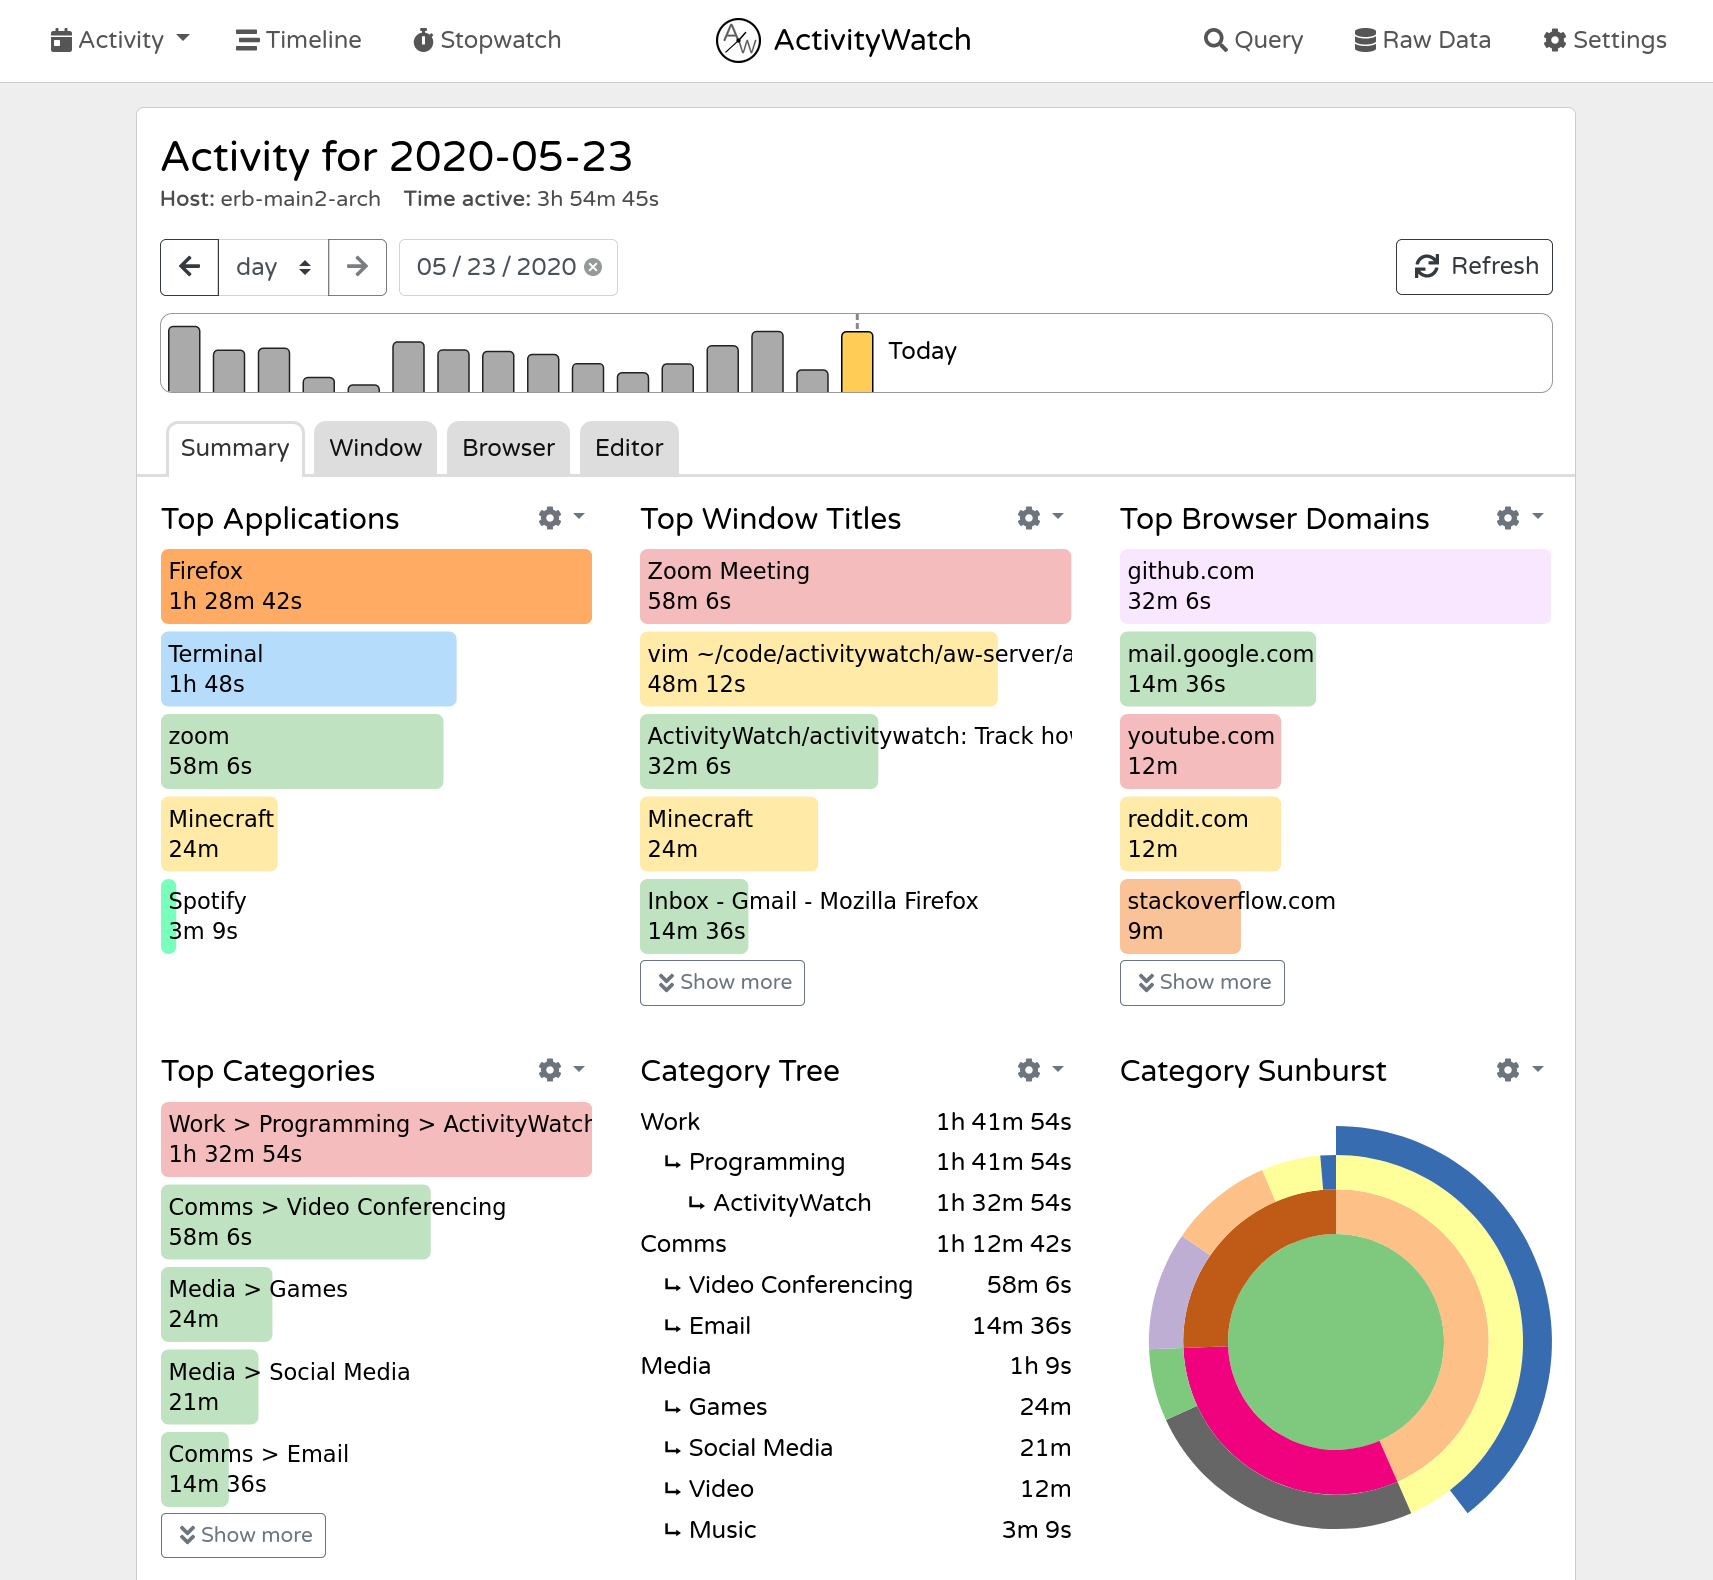
\includegraphics[width=12cm]{img/screenshot-aw-activity.png}
        \caption{ActivityWatch activity dashboard. Showing top applications, window titles, browser domains, and categories.}\label{fig:aw}
        \end{figure}

        ActivityWatch as a project was started in 2016 by the author of this thesis, with his brother Johan joining development soon after. It has since become a popular open source alternative to other time tracking software. It has received numerous contributions from users\footnote{Contributor statistics available at \href{https://activitywatch.net/contributors/}{activitywatch.net/contributors/}} and is approaching 100,000 downloads\footnote{Download statistics available at \href{https://activitywatch.net/stats/}{activitywatch.net/stats/}}.

        \todo[inline]{What more could I add about ActivityWatch? There should be relevant stuff in the docs, and in the slides I made way back.}

\subsection{EEG and low-cost biosensors/functional brain imaging}

    Functional brain imaging methods such as fMRI, fNIRS, and EEG, have been used to study the relationship between cognitive or physical activity, and brain activity~\cite{floyd_decoding_2017}\cite{hong_classification_2015}\cite{fucci_replication_2019}. The more accurate methods such as fMRI are costly and inflexible/impractical for many uses.

    However, the recent availability of low-cost biosensors such as EEG, HEG, and fNIRS, enables studying brain activity during real-life tasks.

    But EEG is not without its limitations --- among them a notably low signal-to-noise ratio~\cite{mcfarland_eeg-based_2017}, as well as being difficult to use for discerning activity deeper in the brain~\cite{fahimi_hnazaee_localization_2020} --- yet these limitations have been overcome for many applications, like ERP experiments, and has even turned out prove sufficient for high-speed BCI applications through detecting visual evoked potentials (VEPs)~\cite{spuler_high-speed_2017}.

    To combat the low signal-to-noise ratio, machine learning methods have been employed with varying degrees of success. Examples from previous research include Convolutional Neural Networks (CNNs), which have been successful in classifying time series in general~\cite{zhao_convolutional_2017}, and EEG data in particular~\cite{schirrmeister_deep_2017}. As well as Hierarchical Convolutional Neural Networks (HCNNs), which have been used for EEG-based emotion recognition~\cite{li_hierarchical_2018}.

    \add[inline]{Separate sections for applications in BCIs vs neuroscience}

    \subsubsection{Cost reduction}

    The cost-reduction of EEG devices took hold in 2013, when OpenBCI ran the founding crowdfunding round on Kickstarter. During the campaign, they offered their 16-channel Cyton + Daisy board for \$549.\footnote{Fun fact: I funded them at one of the lower tiers back then.}\cite{noauthor_openbci_nodate}

    The commercialization of EEG towards a general audience was furthered by InteraXon with the release of the original Muse in 2016. Aimed at meditation practice, it was the first consumer-oriented EEG device on the market.

    More recently, projects like the FreeEEG32 offer a 32 channel board for only \$199, expected to ship in 2022.\cite{noauthor_freeeeg32_nodate}

    \subsubsection{Applications in neurolinguistics}

        EEG has found many applications in neurolinguistics, both to understand how the brain processes natural languages as well as programming languages~\cite{prat_relating_2020}.

         As an example it has been shown that it is possible to classify if a participant is reading code or prose using fMRI~\cite{floyd_decoding_2017}, which has been replicated using EEG and low-cost biosensors~\cite{fucci_replication_2019}. The ability to distinguish between these two tasks have been has been explained neurologically by the recruitment of different neural networks in the brain~\cite{ivanova_comprehension_2020}. 

        The code vs prose comprehension task has also been modified into a writing task studied under fMRI, to further shed light to the underlying brain activity. In one study it was found that code and prose writing are significantly dissimilar tasks for the brain, where prose writing engages brain regions associated with language in the left hemisphere while while code writing engages brain regions associated with attention, working memory, planning, and spatial cognition in the right hemisphere\cite{noauthor_neurological_nodate}. To study this with MRI, the authors had to use (develop?) an MRI-safe keyboard.

        As far as I know, code vs prose writing has not been studied with EEG\. However, using ActivityWatch and other tools we've developed in this thesis (like the input watcher) one can to distinguish wether the user is reading or writing, as well as wether they're working with code or prose, which enables studying the same activities in a naturalistic setting.

    \subsubsection{Applications in software engineering}

        \add[inline]{Applications to software engineers (Fucci and related stuff)}

    % https://docs.openbci.com/citations

    % List of functional brain imaging techniques:
    %  - fMRI
    %  - fNIRS
    %  - EEG
    %  - HEG

\subsection{Aim of the thesis}

    The primary aim of the thesis is to improve upon previous attempts~\cite{fucci_replication_2019} to classify whether the user is reading code or prose using EEG data. This is to be achieved by using better EEG equipment and state of the art analysis methods such as Riemannian geometry. A secondary aim of the thesis is to investigate whether the ability of EEG analysis to classify code vs prose comprehension generalizes across more activities, such as the wide variety of tasks engaged in during organic device use.

    Secondary aims of the thesis include:

    \begin{enumerate}
        \item Implementing a classifier for device activities from EEG data, during organic device use
        \item Improving open-source tools for EEG analysis
    \end{enumerate}

    \add[inline]{Insert stuff from goal document}

\subsection{Related work}

    A systematic mapping study has been published which seeks to review the usage of psychophysiological data in software engineering~\cite{vieira_usage_2021}.

    It has previously been shown that fMRI~\cite{floyd_decoding_2017} and EEG\cite{fucci_replication_2019} provides enough information to classify whether a subject is reading prose or code. However, accuracy with single-channel EEG has been found to be poor, and notably outperformed by a heart rate variability (HRV) monitor.

    % Here, we used functional magnetic resonance imaging to investigate two candidate brain systems: the multiple demand (MD) system, typically recruited during math, logic, problem solving, and executive tasks, and the language system, typically recruited during linguistic processing.
    Recently, it has been shown that the multiple demand (MD) system is typically recruited for code comprehension tasks, as opposed to the language system that is typically recruited during prose comprehension~\cite{ivanova_comprehension_2020}. This sheds light on the significant differences in how the brain processes code vs prose.

    In addition to purely studying comprehension (reading) code and prose, an 2020 fMRI study showed that there are indeed significant neurological differences between \emph{writing} code and prose as well~\cite{noauthor_neurological_nodate}.

    In software engineerig research, low-cost biosensors such as wristbands that measure electrodermal activity and heart-related metrics have been used for emotion detection, as a tool in studying developer productivity.

    \add[inline]{Insert mention of preprint that Fucci mentioned?}
